\chapter{Report Body} \label{Body}
%The central part of the report usually consists of three or four chapters detailing the technical work undertaken during the project. {\bf{\textcolor{red}{The structure of these chapters is highly project dependent}}}. They can reflect the chronological development of the project, e.g. design, implementation, experimentation, optimisation, evaluation, etc (although this is not always the best approach). However you choose to structure this part of the report, you should make it clear how you arrived at your chosen approach in preference to other alternatives. In terms of the software that you produce, you should describe and justify the design of your programs at some high level, e.g. using OMT, Z, VDL, etc., and you should document any interesting problems with, or features of, your implementation. Integration and testing are also important to discuss in some cases. You may include fragments of your source code in the main body of the report to illustrate points; the full source code is included in an appendix to your written report.

In this chapter, I will explain how each of my chosen algorithms work, and how I went around implementing them as a surface-level explanation. I will then briefly compare what challenges I faced for each of my implementations, and how they compare, both performance-wise and with regards to the kinds of layouts they produce, again as surface-level explanations. I go into greater detail on my implementations in the Implementation section (chapter \ref{Implementation}), how the level layouts generated in each algorithm compare with each other in the Design \& Specification section (chapter \ref{Design}), and how each implementation compares overall (and also performance wise) in the Evaluation section (chapter \ref{Evaluation}). For this project, I chose to use the following 4 algorithms.

\begin{enumerate}
    \item Lindenmayer Systems (or L-Systems)
    \item Perlin/Simplex Noise
    \item Poisson Disk Sampling
    \item Voronoï Cells
\end{enumerate}

All of the above algorithms are ``ontogenetic." This means that it attempts to recreate the final steps of a real-world process or mathematical calculation without going through much of the intermediary steps.\cite{pcgwikionto} This contrasts with ``telelogical" procedural generation algorithms, which \textbf{directly} simulate and/or model part of the real world as part of its content generation.\cite{pcgwikitele} This difference between them is described very well in a 2008 article for video games magazine Gamastura by Mick West:

``Two competing methodologies in procedural content generation are teleological and ontogenetic. The teleological approach creates an accurate physical model of the environment and the process that creates the thing generated, and then simply runs the simulation, and the results should emerge as they do in nature.

The ontogenetic approach observes the end results of this process and then attempts to directly reproduce those results by ad hoc algorithms. Ontogenetic approaches are more commonly used in real-time applications such as games. (See "Shattering Reality,"[sic] Game Developer, August 2006.)"\cite{teleonto}\cite{shatteringreality}\cite{randomscattering}

\section{Algorithms}

In this section, I will explain how each of the algorithms I implemented work, then I will go into small detail as to how I implemented them. I go into further detail in the ``Implementation" section of this report.

\subsection{Lindenmayer Systems} \label{alglsys}

Hungarian academic Aristid Lindenmayer devised a mathematical model for the reproduction of fungi in 1967.\cite{LINDENMAYER1968300} His model involved a string of symbols, each unique symbol denoting a specific action and/or branch. Essentially, running that initial string, called the \emph{axiom}, through a set of rules (called a \emph{grammar}) gives us an ever-expanding string that is then taken as instructions to draw something from. Lindenmayer Systems, or L-Systems, have since been used in several scenarios beyond its initial purpose of modelling fungi, from trees to fractals. In video games, they are frequently used to aid in the creation of foliage in several environments, as well as buildings and, here, level layouts. I go over how I got my implementation to work with complex multi-rule grammars in Chapters \ref{implsys1} and \ref{implsys2}.

\subsubsection{A Basic 0L-System} \label{lbasic}

The most basic form of L-System is a \emph{0L}-System, 0 in this case referring to the fact that the grammar is \emph{context-free}.

For this example\cite{lsyspaulbourke}, consider an alphabet $V$, which consists of the following symbols:

\newcommand{\F}{\mbox{F}}

$$ \F, +, - $$

where $\F$ means ``to go forward", and $+$ and $-$ denote turning right or left (respectively) a set number of degrees \o.

Take an axiom $\omega$, for example:

$$ \F+\F+\F+\F $$

And a set of rules $P$ which, in this case, is of size 1:

$$ \F \rightarrow \F+\F-\F-\F\F+\F+\F-\F $$

We can represent this \emph{parametric} L-system in the following form:\cite{houdinilsystems}

$$ G = (V, \omega, P) $$

The first 3 iterations of string replacement with this one-rule grammar $G$ are shown here:

\begin{figure}[H]
	\centering
	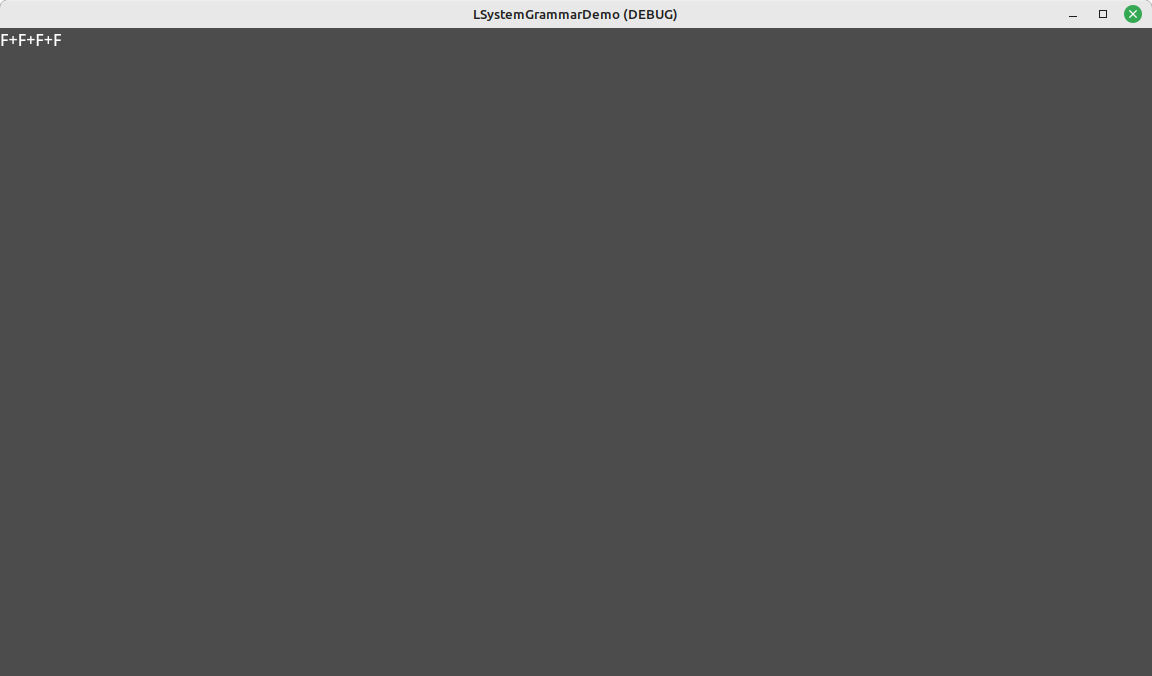
\includegraphics[width=0.5\textwidth]{Images/initial-l-system-iteration-0.png}
	\caption{The axiom of the aforementioned simple L-System with just one rule. String size: 8.\\Source: Own work.}
	\label{fig:lsysiter0}
\end{figure}

\begin{figure}[H]
	\centering
	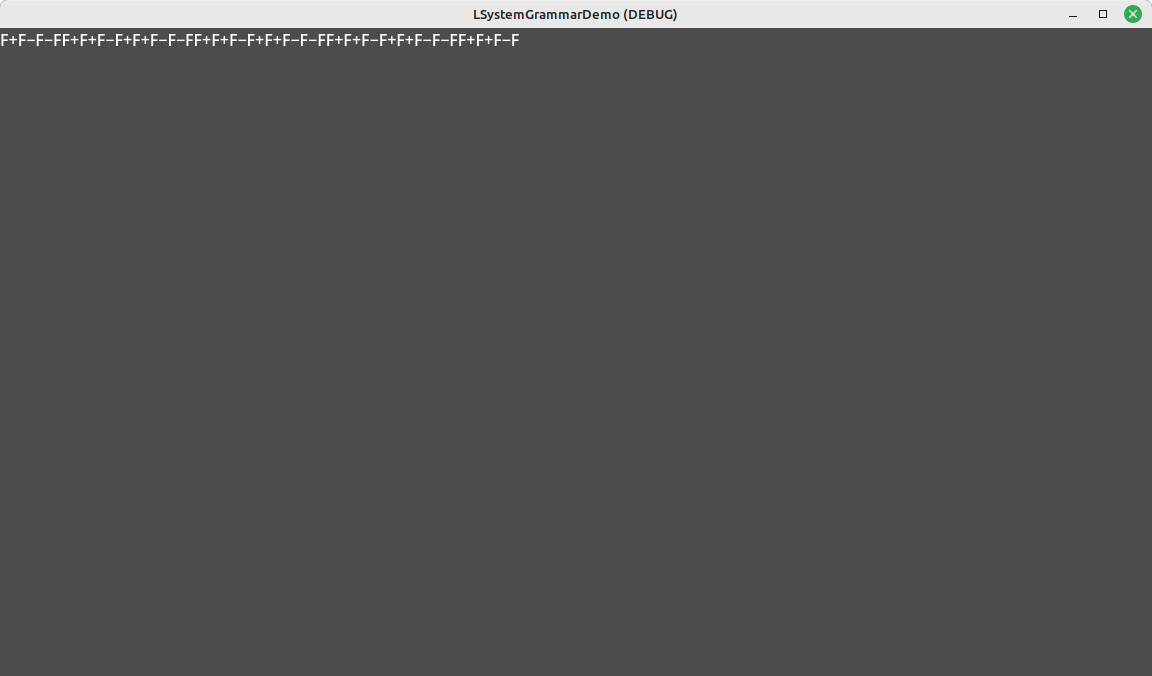
\includegraphics[width=0.5\textwidth]{Images/initial-l-system-iteration-1.png}
	\caption{The first iteration of the aforementioned simple L-System with just one rule. String size: 59.\\Source: Own work.}
	\label{fig:lsysiter1}
\end{figure}

\begin{figure}[H]
	\centering
	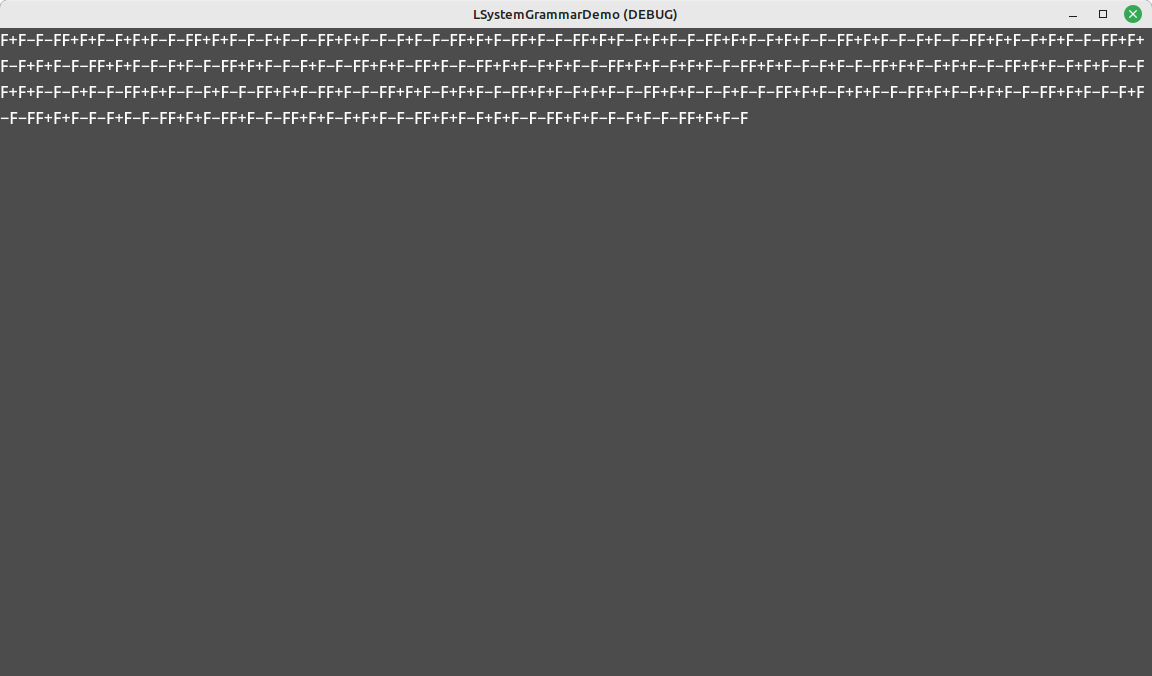
\includegraphics[width=0.5\textwidth]{Images/initial-l-system-iteration-2.png}
	\caption{The second iteration of the aforementioned simple L-System with just one rule. String size: 475.\\Source: Own work.}
	\label{fig:lsysiter2}
\end{figure}

\begin{figure}[H]
	\centering
	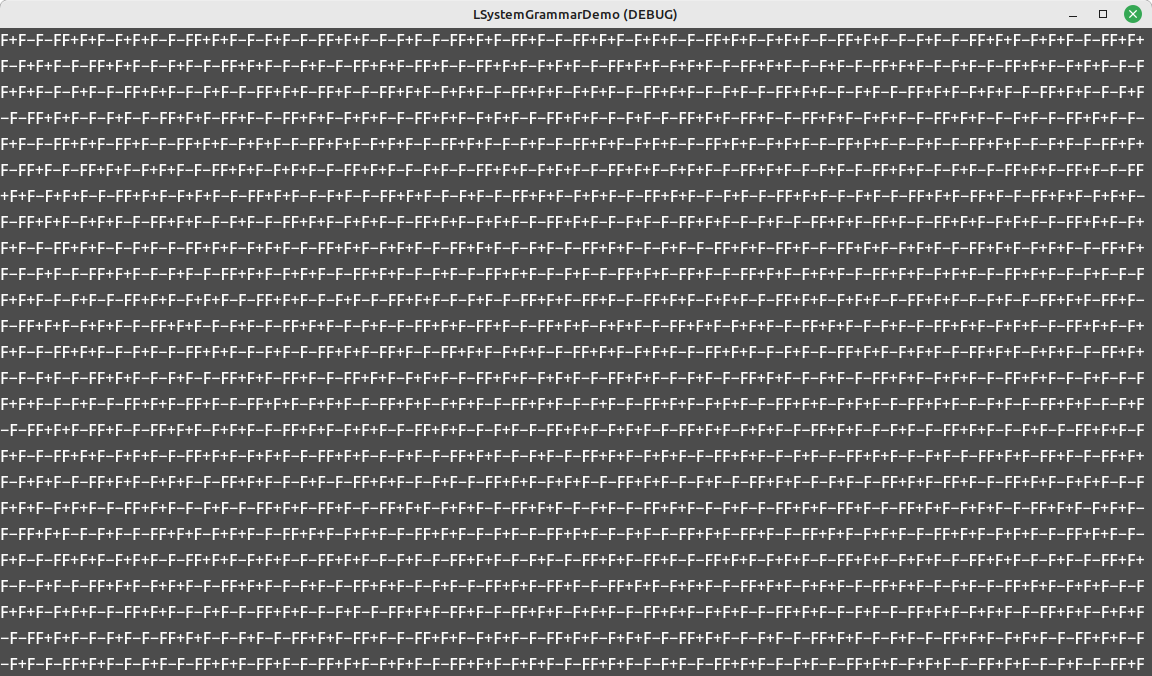
\includegraphics[width=0.5\textwidth]{Images/initial-l-system-iteration-3.png}
	\caption{The third iteration of the aforementioned simple L-System with just one rule. String size: 3803. The string is too large to show in the window, as you can see here.\\Source: Own work.}
	\label{fig:lsysiter3}
\end{figure}

The resulting string can be used to draw a lattice.\cite{lsyspaulbourke} Examples of the above grammar in action are below.

\begin{figure}[H]
    \centering
    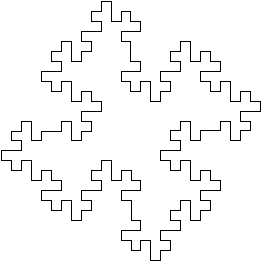
\includegraphics[height=0.25\textheight]{Images/lsys03.png}
    \caption{A lattice generated with the example grammar on a custom-written Classic Mac OS application specifically written for working with L-Systems.\cite{lsyspaulbourke}}
    \label{fig:lattice1}
\end{figure}

\begin{figure}[H]
    \centering
    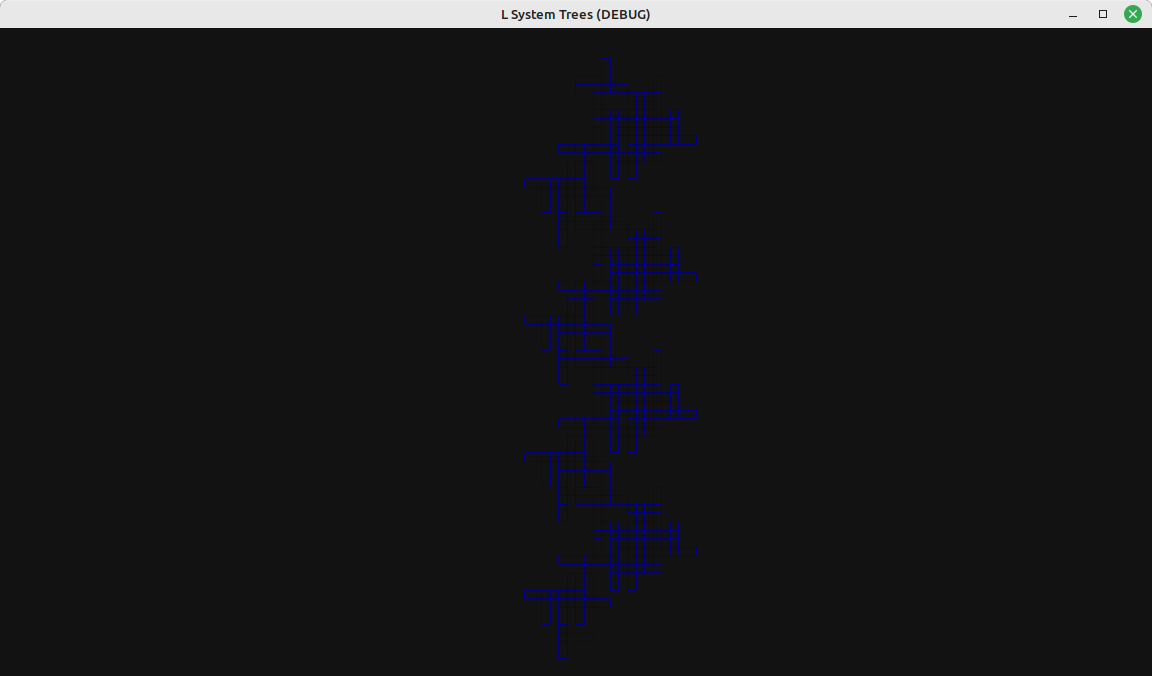
\includegraphics[width=0.75\textwidth]{Images/gd4lattice.png}
    \caption{A lattice generated with the example grammar on a Godot project for drawing from L-Systems. Source: Initial project written by Alexander Gillberg for his YouTube channel Codat\cite{codatGD3LSystemYT}\cite{codatGD3LSystemGH}, and converted to Godot 4 (with the addition of the lattice grammar) by the author of this report.\cite{codatGD4LSystemGH}}
    \label{fig:lattice2}
\end{figure}

\subsubsection{A More Complex D0L-System With More Than One Rule} \label{lcomplex}

The grammar in the following example represents a D0L-System\cite{lsystemintro}, a \textbf{deterministic} L-System using a context-free grammar; the grammar in the first example was \textit{also} deterministic.

\newcommand{\A}{\mbox{a}}
\newcommand{\B}{\mbox{b}}

For this example, consider a new grammar $G$ with the alphabet $V$, where $\A$ and $\B$ are the only symbols. We start with the following axiom $\omega$, which is just $\A$. We now have a set of rules $P$ which is, this time, of size \textit{2}:

$$ \A \rightarrow \A\B $$
$$ \B \rightarrow \A $$

The first few steps of the resulting derivation can be modelled like so:

\begin{figure}[H]
    \centering
    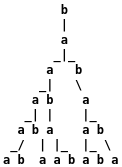
\includegraphics[scale=0.5]{Images/derivationtree.png}
    \caption{The first few steps of a derivation of our example grammar.\cite{lsystemintro}}
    \label{fig:derivationtree}
\end{figure}

\subsection{Perlin/Simplex Noise}

Traditionally, white noise images, and most other noise types, place noise pixels completely randomly, without each pixel considering the values of its neighbours\cite{gd3perlinnoise}, as you can see in Figure \ref{fig:whitenoisepic}.

However, there exists several types of \textbf{value} and \textbf{gradient} noise that \textit{do} take surrounding pixel values into consideration, and will therefore serve more use in building levels in our games.

Value noise simply takes a lattice of points with random values and then interpolates those points based on their surrounding values. This \textit{can} be used as a procedural texture. However, due to the simple nature of the algorithm, it's possible that the difference between several values in a region is minimal, while in other regions the values may differ immensely, resulting in a noise image that is not very smooth.

Gradient noise, on the other hand, takes point lattices and instead calculates the interpolation between tangents.\cite{perlinvalue} Since both tangents between a curve must be collinear\cite{perlinvalue}, the flat and bumpy curves produced by value noise's interpolation calculations are now much less likely to be returned, as seen in Figure \ref{fig:valueperlincomparison}.\cite{perlinvalue} This results in noise images of higher and more appealing visual quality as, to quote a response from Stack Exchange by Hernan J. González\cite{gradientvalue}, ``it cuts low frequencies and emphasizes frequencies around and above the grid spacing."

\begin{figure}[H]
    \centering
    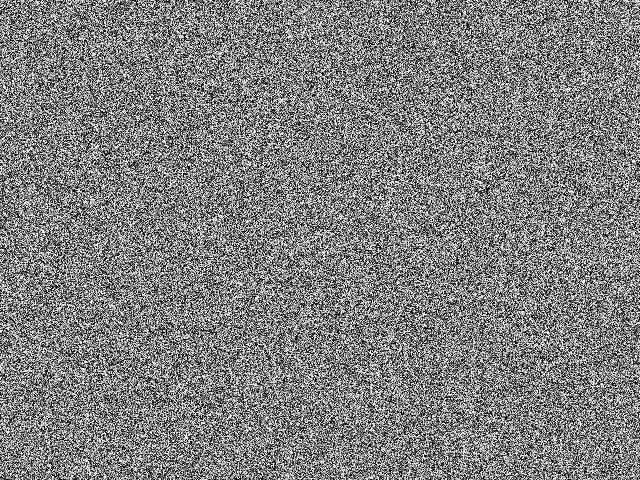
\includegraphics[width=0.75\textwidth]{Images/whitenoisepic.png}
    \caption{A white noise picture generated with Robson's white noise image generator.\cite{whitenoisepicgen}\\Settings: 640 squares horizontally, 480 squares vertically, size of squares 1, colours greyscale, bias none.}
    \label{fig:whitenoisepic}
\end{figure}

\begin{figure}[H]
    \centering
    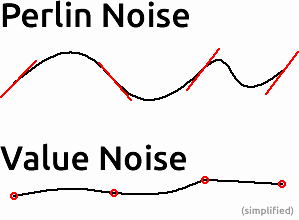
\includegraphics[width=0.75\textwidth]{Images/valueperlincomparison.png}
    \caption{A comparison between the kinds of curves produced by Value noise interpolation and Perlin (and other Gradient) noise interpolation.\cite{perlinvalue}}
    \label{fig:valueperlincomparison}
\end{figure}

Two particularly well-known Gradient noise algorithms that are commonly used for procedurally generating levels are the already mentioned Perlin Noise and Simplex Noise, both designed by American Computer Science professor Kenneth H. Perlin, with the former being an improvement on the former. Perlin Noise also takes a lattice of randomly assigned gradients, but the algorithm interpolates the dot products of those points instead of just their neighouring values.\cite{fastnoiselitedocs} Simplex noise, meanwhile, tries to reduce the grid artifacts caused by the original algorithm, and has the added benefit of scaling better to larger dimensions.\cite{pcgwikisimplex} Perlin filed a patent on his work in 2002 that was granted in 2005\cite{perlinpatent}, which prompted the creation of the OpenSimplex noise algorithm\cite{opensimplex}\cite{simplexarticle1}\cite{simplexarticle2} for free use; the patent has since expired in 2022, allowing free use to both Perlin and the original Simplex noise.\cite{perlinpatent}

Godot 3 previously featured an OpenSimplexNoise class\cite{opensimplexdocs}\cite{gdblogsimplex} for generating noise textures, which used the OpenSimplex algorithm. In addition to using a ``simplectic honeycomb" for its lattices\cite{simplexarticle2}, this algorithm also  (to quote Michael Powell) ``expands the range of the gradients a bit, so they can extend a little bit into neighboring cells. This theoretically makes the noise a little bit smoother, but it also means that extra cells need to be checked."\cite{simplexarticle1} Godot 4, on the other hand, allows us to use the \textit{original} Simplex noise algorithm, as well as Perlin noise, 2 types of Value noise and a variation of Simplex noise that produces smoother, high quality noise images with an additional performance cost, and it allows us to control which algorithm we use for noise generation using the ``noise\_type" property and ``NoiseType" enumeration in the ``FastNoiseLite" class that is now used for noise.\cite{fastnoiselitedocs} 

\subsection{Poisson Disk Sampling}

Poisson disk distributions are an easy way to randomly scatter objects across a field. It's commonly used for tree placement and placement of other random objects. Points are placed over a plane, with a single point placed randomly and subsequent points calculated such that a single point has no other point lying within a given radius of said point. Different implementations of Poisson disk distributions or samples can accommodate multiple radii for points in a plane, and some implementations produce \textit{maximal} samples- that is, a set of samples that fully cover the given plane, while still adhering to the principle that no single point has other points lying within its radius\cite{10.1145/1964921.1964944} (the implementation I made for this project does \textbf{not} guarantee maximality, however).

An implementation of Poisson disk sampling was originally developed in 1991 by Don P. Mitchell\cite{10.1145/127719.122736} as a replacement for inefficient Monte Carlo ``dart-throwing" algorithms.\cite{pdshistory} Mitchell's algorithm ran in $\mathcal{O}(n^{2})$ time, whereas Robert Brinson's 2007 improved algorithm for Poisson disk sampling\cite{10.1145/1278780.1278807} ran in $\mathcal{O}(n)$. Subsequent quality and speed improvements to Brinson's algorithm were published in 2019\cite{pdsimprovementroberts}, 2021\cite{pdshistory} and 2022\cite{pdsimprovementrus}. The implementation made for this project, as well as the Unity project I based it on, were both based on Brinson's 2007 $\mathcal{O}(n)$ algorithm.\cite{seblaguetuteGH}\cite{seblaguetuteYT}

The following are some examples of Poisson disk distribution in action:

\begin{figure}[H]
    \centering
    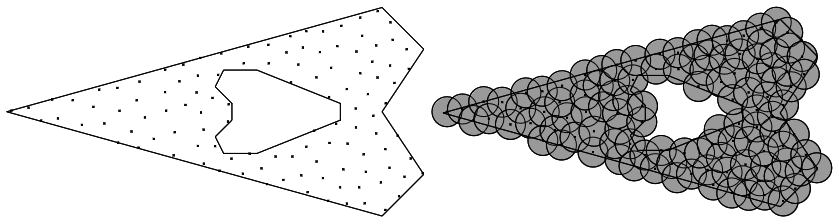
\includegraphics[width=\textwidth]{Images/maximalpoissonsample.png}
    \caption{A diagram of a maximal Poisson disk distribution done on a concave plane, with the right side denoting maximality through the grey disks overlapping but not any points overlapping.\cite{10.1145/1964921.1964944}}
    \label{fig:maximalpoisson}
\end{figure}

\begin{figure}[H]
    \centering
    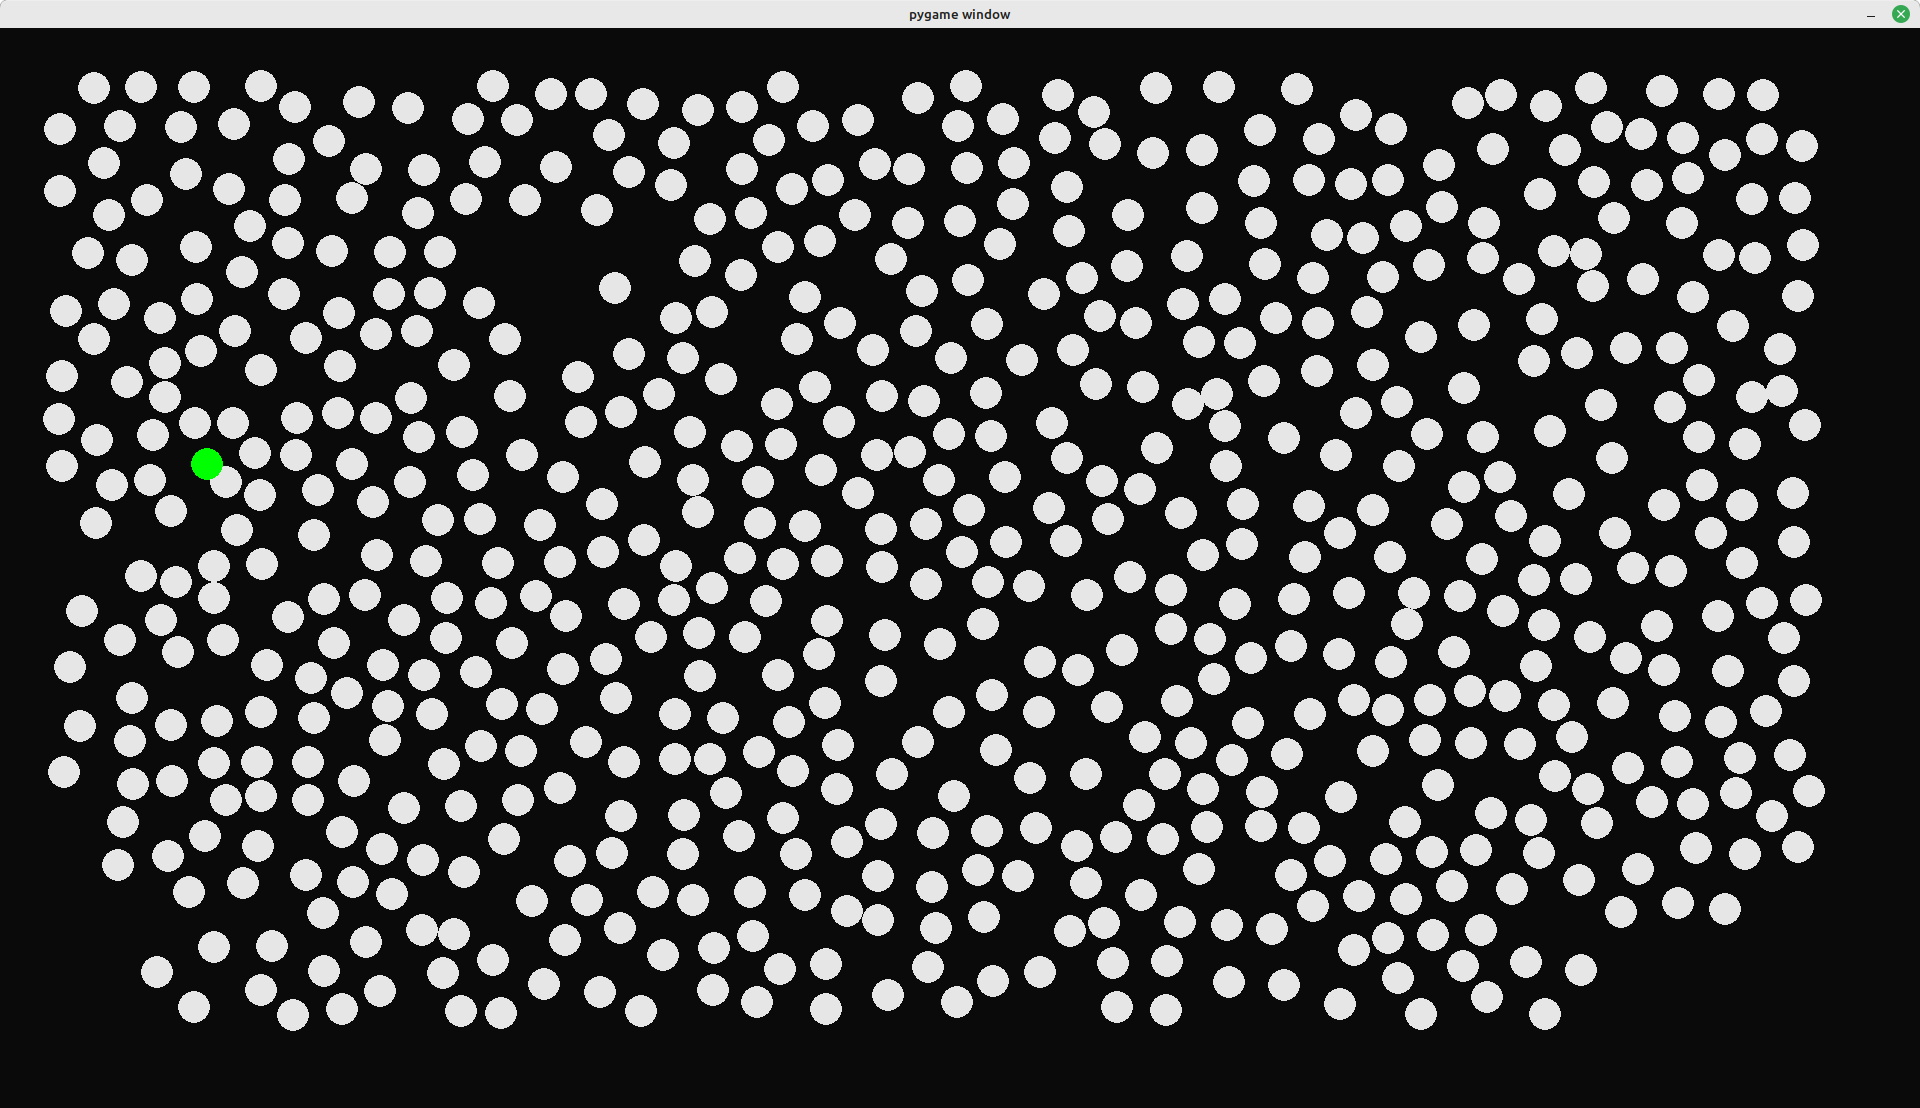
\includegraphics[width=\textwidth]{Images/pygamepoissonsample.png}
    \caption{An implementation of Poisson disk sampling made in Pygame.\cite{pygamepoissondisksampling} The screenshot was taken \textit{after} all of the samples were taken.}
    \label{fig:pygamepoisson}
\end{figure}

\subsection{Voronoï Cells}

Named after the Ukranian mathematician Georgy Voronoy, Voronoï cells work by taking a map of points, and randomly selecting a group of points. Within that selected group, cells are formed by calculating, in each point of the grid, the closest of the selected points to it. That is, each cell represents the group of points that are the closest to that random point (including that point in the group as well).\cite{pcgwikivoronoi} The final arrangement of cells represents a Voronoï Diagram or Voronoï Tesselation.

Distances between points can be calculated with either the Euclidean distance:

$$ d_{E}(p, q) = \sqrt{(q_x - p_x)^2 + (q_y - p_y)^2} $$

or the Manhattan distance:

$$ d_{M}(p, q) = |q_x - p_x| + |q_y - p_y| $$

With the Euclidean distance producing a more ``triangulated" tesselation than the Manhattan distance, with straighter diagonals and cells shaped like irregular polygons, the geometry of which is more "blocky" and resembles taxicabs (hence its alternate name "Taxicab Geometry"). Two visual comparisons of the kinds of Voronoï cells generated with either distance calculation are shown in Figures \ref{fig:voronoicomparison} and \ref{fig:secondvoronoicomparison}.

\begin{figure}[H]
    \centering
    \includegraphics{Images/Voronoitessellations.jpg}
    \caption{A visual comparison of the kinds of Voronoï cells generated with the Euclidean and Manhattan distance.\cite{reffortesselations}}
    \label{fig:voronoicomparison}
\end{figure}

\begin{figure}[H]
    \centering
    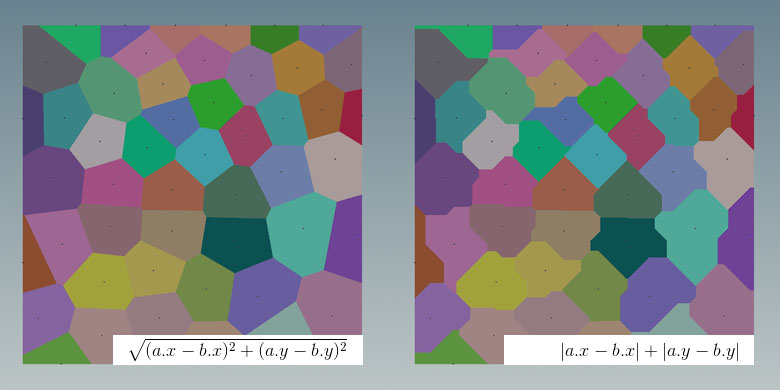
\includegraphics[width=\textwidth]{Images/manhattan_example_02.jpg}
    \caption{Another example of the differences between a Voronoï tesselation with distance between points calculated with either the Euclidean distance or the Manhattan distance.\cite{manvoronoi}}
    \label{fig:secondvoronoicomparison}
\end{figure}

\section{Implementations}

Here I will describe, at surface level, the methods I went about implementing the above algorithms and what references I used.

\subsection{Commonalities Between Implementations} \label{commonalities}

To implement the same scenario, aforementioned in the background of this report, across all 4 algorithm implementations, I had to include some of the same code and functions, as well as the same tile set shown in Figure \ref{fig:kenneyset}.

From this tileset, which contains 1078 tiles, my code uses 27 building tiles, 13 tiles for trees and other fauna, 1 tile for the player character and one of 4 tiles for the ring. The relevant coordinates of the tiles for buildings, trees and the ring are each stored in constant arrays in the script, while the player tile's coordinates are just stored in a local constant (not an array, since there is no need for one).

To handle player placement and subsequent movement, I have several functions. Godot's built in ``physics\_process" function handles events that happen in real-time, and is commonly used, like in this context, for player movement. In it, I first store the current player's cell, ``player\_movement\_cell", in ``previous\_cell", then I initialise a ``direction" based on which input movement was pressed (``Vector2i.LEFT" when ``"ui\_left"" was pressed, and so on). Then I add the player's current cell with the direction to calculate the potential ``new\_movement\_cell". If this cell is within the bounds of the enviroment, as well as either a tree or empty space (or the ring), it moves there, and the previous cell gets erased. If the player ends up moving into the cell where the ring is, the player wins the game, and all movement is paused while a winner's dialog popup shows up. The player moves \textbf{very} quickly in our games, and I have yet to figure out how to slow down this movement while also not making movement so slow that the games drags; the player will not want to have to continually press down an arrow key to move to 1 cell in a map of 2880 cells. Since the performance of the algorithms are more important in this project, however, I decided to leave the very fast player movement as is.

I have written ``place\_player" and ``place\_ring" functions that handle the random generation of the player's and ring's initial starting positions. Both use the ``\_get\_random\_placement\_cell" helper function to retrieve a new cell, and both use a while loop to make sure the randomly generated cell isn't already occupied. In both functions the placement cells are assign and calculated \textbf{before} the while loop, so that their placements do not default to just (0, 0) in the beginning.

\begin{figure}[H]
    \centering
    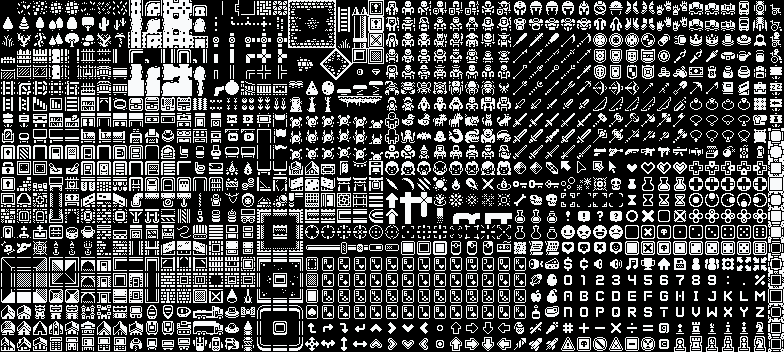
\includegraphics[width=\textwidth]{Images/monochrome_packed.png}
    \caption{The tileset used for all 4 implementations of my scenario with PCG algorithms.\cite{kenneyassetsused} Of all the 1078 tiles, of size 16x16, in this tileset, only 45 of them get referenced in my code.}
    \label{fig:kenneyset}
\end{figure}

Across all implementations, there are two local variables, ``x\_tile\_range" and ``y\_tile\_range". Both of these calculate the dimensions of our tile map by taking the display window's respective x and y dimensions from the project's settings (1152x640) and divides them by the respective x and y dimensions of the cell size (16x16). ``x\_tile\_range" should resolve to 72 upon runtime, and ``y\_tile\_range" should equal 40, giving us our 72x40 tile map that gives us a total of 2880 cells to work with in our games.

Finally, there are two dialog popups added to each scene tree, one for describing the game's story (``AcceptDialog", of type ``AcceptDialog") and another for when the game ends after the player has collected the ring (``WinDialog", of type ``ConfirmationDialog"). For ``AcceptDialog" the ``confirmed" and ``canceled" signals are both connected to the function ``\_on\_AcceptDialog\_closed", which hides the popup and unpauses the game. For ``WinDialog", on the other hand, ``confirmed" is connected to ``\_on\_WinDialog\_confirmed" and ``canceled" is connected to ``\_on\_WinDialog\_canceled". ``\_on\_WinDialog\_confirmed" is meant to generate a new level layout, while ``\_on\_WinDialog\_canceled" is meant to close the game, both when the cancel button (labelled "Get Me Out of Here") is clicked and when the cross on the top-right corner of the popup is clicked. However, as of now, only the top-right corner of both popups does what it is supposed to; clicking any of the other buttons from both popups, for some reason, does nothing at the moment, and I \textit{did} make sure, in my code, that the signals were properly connected. However, the games themselves still run as they are supposed to, and the integration of the algorithms into the levels in the games are more important here, so since \textit{they} still work, I decided to leave the popups, their behaviour and their code as they were. \textit{If} they are engine issues, regarding the buttons, they may hopefully get fixed in future versions of Godot.

\subsection{Lindenmayer System} \label{implsys1}

The implementation of an L-System was very simple. I took inspiration from a YouTube video on implementing an L-System for drawing line graphics in Godot by Alexander Gillberg.\cite{codatGD3LSystemYT} In the code from the Godot 3 project Gillberg made in that video\cite{codatGD3LSystemGH}\cite{codatGD3LSystemYT}, he created a custom ``Rule" class in GDScript, with which he defined new rules. I forked his project, converted it to Godot 4 and used it to create the lattice graphics in Figure \ref{fig:lattice2}.\cite{codatGD4LSystemGH} I did this mainly as a reference for my implementation of L-Systems in the game itself.

With the implementation in my \emph{game}, I adapted the ``get\_new\_character" method in that L-System to work with the dictionary I originally implemented my L-System in. The new ``get\_new\_replacement" method in my implementation allows for there to be more than one grammar rule while the L-System still performs as it should. My original L-System iterated through the original string \textit{directly}, which produced unintended consequences in grammars with multiple rules, as seen here when trying to implement the D0L-System I mentioned earlier\cite{lsystemintro}:

$$ b \rightarrow a \rightarrow aa \rightarrow aaa \rightarrow aaaa \rightarrow aaaaa \ldots $$

By using an empty string buffer and inserting rule replacements there instead, my implementation is now able to perform substitutions accordingly; the correct computation of the D0L-System is denoted in Figure \ref{fig:derivationtree} and repeated below:

$$ b \rightarrow a \rightarrow ab \rightarrow aba \rightarrow abaab \rightarrow abaababa \ldots $$

With the L-System string parsing algorithm in place, the next step was to paint the cells of each tile. With this, I iterated through every cell of the tilemap using a nested for-loop. With the parsed string, I then accessed the character of the string at an incremented index using an iterator variable I defined before the for-loops. The string consists of three different characters repeated multiple times, ``O", ``W" and ``B". For each string index, if the character is ``W", paint a tree, if it is ``B", paint a building, and if it is an ``O", leave the cell blank and paint nothing. The player and ring then get placed afterwards.

Even for a large-sized tile map with 2880 cells, a constant L-System $G$, with the symbols O, W and B and the following grammar

$$ \mbox{O} \rightarrow \mbox{O}\mbox{W}\mbox{O} $$
$$ \mbox{W} \rightarrow \mbox{W}\mbox{B} $$
$$ \mbox{B} \rightarrow \mbox{B}\mbox{W}\mbox{O} $$

can parse the axiom OWB, paint tile map tiles with the resulting string \textbf{and} place the player and ring in just 19 milliseconds on average. This was the default grammar used by the L-System in the game. I also included 3 more grammars, one that generated more buildings (and impossible level layouts), another that generated more trees and another that generated more empty space. These can be easily selected with the ``ruleset" export variable in the Godot editor. Further variance can be added with the addition of a randomly generated axiom, capped at a maximum height or smaller (minimum 1). If said option is enabled in the Godot editor, the default value in the export variable for setting this cap is 10, and since it is an export variable, it too can be adjusted in the editor as the developer sees fit.

\subsection{Perlin/Simplex Noise} \label{impperlin1}

The Simplex Noise implementation works with Godot's built-in Noise library. Within a Sprite2D node's Texture attribute, I set a new ``NoiseTexture2D" field inside of it. In its ``Noise" attribute I created a new ``FastNoiseLite" scene, which generates a noise texture for us to use. The seed can be set in the sprite's script file.

As with my other implementations, there are two separate arrays, one for trees and another for buildings. For each cell in the TileMap, I then took the noise pixel from the generated texture at that exact point (scaling with the cell size accordingly), using the ``get\_noise\_2d" method built-in with Godot, and then, depending on the value retrieved, decided, firstly, whether or not to place a plant/tree tile there and, secondly, whether or not to place a building tile there. As a result, not every cell in the TileMap has tiles on it. On any one of those empty cells, the Player tile will then get placed.

For the generation of the noise itself, I \textit{could've} added a ``Sprite2D" node to the scene tree, the root of which was my ``TileMap", and gave it a ``NoiseTexture2D" texture and set its ``noise" property to a newly-created ``FastNoiseLite" instance, the latter of which contains the actual noise data. In the early stages of this implementation's development, that's what I did, and I created a script that solely set the seed of the ``FastNoiseLite" resource to a random integer (using the ``randi" method). However, for a more authentic result, and to forgo the need of an additional node and noise texture that will not even be visible in the final product, I decided to create the noise for this algorithm implementation entirely programmatically. I stored the ``FastNoiseLite" instance in its own class variable ``noise", and instantiated it with the ``set\_noise" method when starting the game (the ``\_ready" function automatically runs when the game starts).

Initially having done the noise integration with a sprite node and noise texture allowed the author of this report to experiment with some of the ``FastNoiseLite" class's properties before finally resorting to programmatic noise creation. An instance of this class, by default, uses the ``Simplex Smooth" noise algorithm, a version of the Simplex algorithm that produces higher quality noise images at the expense of slower speed.\cite{fastnoiselitedocs} We can also use just ``Simplex" noise for higher speed, as well as the original ``Perlin" noise algorithm.\cite{fastnoiselitedocs} Godot also allows us to use two kinds of Value noise, as well as a ``Cellular" type that combines algorithms like Worley Noise and Voronoï diagrams to create "regions of the same value."\cite{fastnoiselitedocs} I had problems with the ``Cellular" noise type when experimenting with it, for reasons I will get into later, but the other noise types I made readily accessible in an ``export" variable in my script (that is, a variable that can be easily accessed in the Godot editor when the TileMap node is clicked on) when I removed the sprite node and decided to programmatically make the noise. When the ``set\_noise" function is called, the noise type is assigned through the ``\_get\_noise\_type" function, which returns an integer value depending on the type of noise selected, and the returned result is cast to ``FastNoiseLite"'s ``NoiseType" enumeration\cite{fastnoiselitedocs} before it gets assigned (this prevents an ``INT\_AS\_ENUM\_WITHOUT\_CAST" warning from the Godot editor's linter for GDScript\cite{projectsettingsdocs}).

Furthermore, I have 3 other export variables in the TileMap script for this implementation that directly correlate to some of ``FastNoiseLite"'s properties. The ``noise\_frequency" variable in the script correlates to the ``frequency" property in ``FastNoiseLite", which, as both names suggest, sets the noise frequency; the higher the frequency, the rougher and more granular the noise\cite{fastnoiselitedocs}, which is probably why it is set to 0.01 by default.\cite{fastnoiselitedocs}  The ``fractal\_type" and ``cellular\_distance\_type" in the script \textbf{directly} correspond to the ``fractal\_type" and ``cellular\_distance\_function" properties respectively, to the point where both even use the relevant enumerations from ``FastNoiseLite" directly (``FractalType" and ``CellularDistanceFunction" respectively).\cite{fastnoiselitedocs} The relevant values are all assigned accordingly in ``set\_noise".

In terms of determining whether or not to place buildings or trees (or nothing), I took inspiration from a YouTube tutorial by Gingerageous Games utilising Godot 3\cite{gingergd3tutorialYT}\cite{gingergd3tutorialGH} (which breaks in Godot 4). His tutorial used multiple ``TileMap" nodes in a single scene tree with a ``Node2D" root, and controlled each individual tile map, representing a specific part of the environment (such as grass and roads), and used a floating point ``cap" to determine whether or not to place a tile in a cell based on the noise pixel retrieved at that cell's coordinate.\cite{gingergd3tutorialYT}\cite{gingergd3tutorialGH} Since I'm using just one tile map for everything (trees and buildings), I had to mitigate a conflict where the building cap was smaller than the tree cap. If that were the case then, since the tree cells get painted first in my implementation, no buildings would ever get painted. To mitigate this, I added an additional condition to my if-statement for painting building cells (in the same line, to prevent creating a nested if-statement), which would allow the algorithm to overwrite an already painted tree cell with a building cell subject to a randomly generated floating point number (between 0 and 1 inclusive) being below a pre-defined floating point number in the exported variable ``building\_overtakes\_tree". This would then allow there to be a controlled proportion of buildings compared to trees (the higher the proportion, the more buildings compared to trees), regardless of whether the building cap was lower than the tree cap or not, and the algorithm would still perform as normal should the reverse be the case.   

\subsection{Poisson Disk Sampling}

The Poisson Disk Sampling implementation was based on a Unity tutorial by Sebastian Lague\cite{seblaguetuteYT}\cite{seblaguetuteGH}, in which he used his algorithm to draw points onto a grid. He based his algorithm on Bridson's $\mathcal{O}(n)$ algorithm.\cite{10.1145/1278780.1278807} The way he wrote \textit{his} implementation was such that the radius of the circle would be equal to the diagonal of each square in the grid by default (when the radius was 1.0), ensuring that no point ever lies within the radius of another.

My implementation of the Poisson Disk Sampling algorithm mostly took from him, with some changes. Lague did his implementation in the C\# language and, while Godot 4 \textit{does} have a separate version with C\# and .NET support, I opted to use the standard GDScript distribution of Godot 4 with all of my implementations. This meant that I had to adapt the code to work with not just the tile map but also the way GDScript worked. For one thing, the ``grid" array in the ``generate\_points" had to be manually initialised by inserting arrays into an empty array, the quantity determined by what would have been the outer length of the 2D array (and what basically \textit{was} this in Lague's implementation), that being the ceiling function of the x-dimension of the sample region size divided by the cell size. From there, in each of the nested arrays, the value 0 had to be programatically inserted to all of them, the quantity of the \textit{zeroes} also being determined by what would have been the \textit{inner} length of the 2D array (and what basically \textit{was} this in Lague's implementation), that being the ceiling function of the y-dimension of the sample region size divided by the cell size.

Adapting Lague's implementation from C\# and Unity to GDScript and Godot involved some extensive research into Unity's API. When calculating the angle in ``GeneratePoints"/``generate\_points", for example, the equivalent of Unity's ``Random.value" in Godot is ``randf" (which \textit{has} no static class to be called from). Furthermore, GDScript has a ``TAU" constant that does the ``Mathf.PI * 2" calculation done in Lague's Unity implementation. The ``sqrMagnitude" method used in Lague's ``isValid" function becomes ``length\_squared" in my ``is\_valid" method. When implementing ``isValid" in GDScript I also had to make sure the inner and outer dimensions of the grid could be adequately accessed. I go over how I did that in the ``Implementation" section of this report (see chapter \ref{Evaluation}).

\subsection{Voronoï Cells} \label{voronoi1}

I based my implementation of this algorithm on some JavaScript code posted by an anonymous contributor to the Procedural Content Generation Wiki on the Wikidot platform in 2017, in which a brute-force implementation of the algorithm was implemented.\cite{pcgwikivoronoi} An auxiliary function in the JavaScript code, ``randRange", was taken out of \textit{this} implementation, since Godot has a built-in ``randi\_range" function that serves the exact same purpose.\cite{gdscriptdocs} As I got further and further with my implementation of Voronoï diagrams in Godot, I realised the way the algorithm inherently worked meant that the level layouts it designed would be wholly unique, espcially compared to the other three algorithms for which I made implementations of my scenario.

For example, unlike the other implementations, the algorithm ensure that all cells of the tilemap were \textbf{always} covered (to start with, in our game's context), whereas the other implementations always left some cells unpainted. The nature of Voronoï tessellations also meant that groups of trees and buildings were bunched together, with no guarantee that they would ever form coherent connections that would make sense in a level of our scenario. This meant that the ring and player placements had to be altered so that, instead of being placed in non-existent empty cells, they would replace the cell of a tree.

Even \textit{with} that, there would be no guarantee that a player would be able to complete a level successfully. For example, if a player and ring were spawned in different Voronoï cells of trees, and both of those cells were separated by cells of buildings such that they could not ever be feasibly reached, the game would be impossible to finish. Therefore, a new input event was created, ``reset\_position", which can be triggered by pressing \textit{either} the G key on a standard computer keyboard \textit{or} the right-click mouse button. Triggering the event respawns the player character in a different position, which could be occupied by either a tree or the ring, ensuring that the ring can still be collected and, therefore, game can still be won. The code for when this event is triggered is essentially a rehash of the code for ``place\_player", except that the new cell \textbf{can} be the cell occupying the ring, and also the previous cell's contents will be deleted (as the player is no longer at that position).

While the differences are drastic and very noticeable, I nonetheless kept working on this implementation and included it in my project. I believe that the fact that I was able to work through it and implement a working version of my scenario with it (albeit with some changes) adds further strength to my claims that Godot can work well with procedural generation algorithms, even ones where use in the context of a tile map RPG would be rarer, as well as proving my strengths as a games programmer in making tile maps work with PCG algorithms.

\begin{figure}[H]
    \centering
    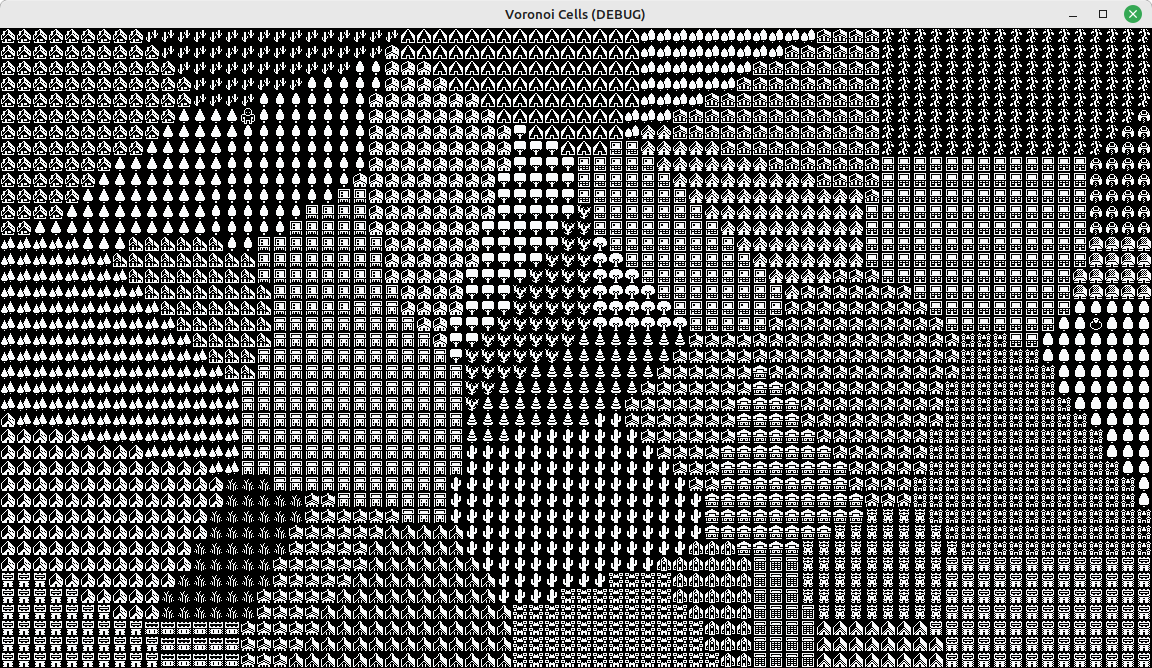
\includegraphics[width=\textwidth]{Images/voronoi-example.png}
    \caption{An example of the Voronoï cells implementation of the scenario in action.}
    \label{fig:voronoi-example}
\end{figure}
